\documentclass[12pt]{article}

\usepackage[utf8]{inputenc}
\usepackage{amsmath, amssymb, amsthm, amsfonts}
\usepackage{graphicx}
\usepackage{tikz}
\usetikzlibrary{decorations.markings} % Required for arrows on paths
\usepackage{geometry}
\geometry{a4paper, margin=1in}
\usepackage{hyperref} % For \url command

% Theorem environments
\newtheorem{theorem}{Theorem}[section]
\newtheorem{lemma}[theorem]{Lemma}
\newtheorem{corollary}[theorem]{Corollary}
\newtheorem{definition}[theorem]{Definition}
\newtheorem{proposition}[theorem]{Proposition}
\newtheorem{remark}[theorem]{Remark}
\newtheorem{example}[theorem]{Example}

% Custom commands
\newcommand{\R}{\mathbb{R}}
\newcommand{\Z}{\mathbb{Z}}
\newcommand{\N}{\mathbb{N}}
\newcommand{\C}{\mathbb{C}}
\newcommand{\Q}{\mathbb{Q}}
\newcommand{\T}{\mathbb{T}} % The Torus R/Z

\title{Weyl's Equidistribution Theorem}
\author{Kai Chen\thanks{Department of Mathematics, Southern University of Science and Technology}}
\date{May 27, 2025}

\begin{document}
\maketitle

\section{Introduction: The Problem of Uniform Distribution}

\begin{definition}[Integer and Fractional Parts]
For any real number $x \in \R$:
\begin{itemize}
    \item The \textbf{integer part} of $x$, denoted $[x]$, is the greatest integer less than or equal to $x$.
    \item The \textbf{fractional part} of $x$, denoted $\langle x \rangle$, is defined as $\langle x \rangle = x - [x]$.
\end{itemize}
Note that $\langle x \rangle \in [0,1)$ for all $x \in \R$.
\end{definition}

\begin{definition}[Congruence Modulo 1]
Two real numbers $x, y \in \R$ are said to be \textbf{congruent modulo 1} (or modulo $\Z$) if their difference is an integer, i.e., $x - y \in \Z$. We write this as $x \equiv y \pmod{1}$.
Equivalently, $x \equiv y \pmod{1}$ if and only if $\langle x \rangle = \langle y \rangle$.
The set of equivalence classes $\R/\Z$ can be identified with the interval $[0,1)$ or the unit circle $\T$.
\end{definition}

Imagine scattering points in an interval. Do they spread out evenly, or do they cluster in certain areas? This question of "uniform distribution" or "equidistribution" is central to many areas of mathematics. Weyl's Equidistribution Theorem provides a profound answer for a specific type of sequence: the fractional parts of multiples of an irrational number.

We are interested in the sequence of fractional parts $\{\langle n\gamma \rangle\}_{n=1}^\infty$.
\begin{proposition}
For any real number $\gamma \in \R$:
\begin{itemize}
    \item If $\gamma \in \Q$, the sequence $\langle n\gamma \rangle$ takes on only finitely many distinct values.
    \item If $\gamma \notin \Q$, the values $\langle n_1\gamma \rangle$ and $\langle n_2\gamma \rangle$ are distinct for $n_1 \neq n_2$.
\end{itemize}
\end{proposition}
\begin{proof}
(i) If $\gamma = p/q$ where $p,q \in \Z, q \neq 0$, then $\langle (n+q)\gamma \rangle = \langle n\gamma + p \rangle = \langle n\gamma \rangle$. The sequence is periodic with period $q$.
(ii) If $\langle n_1\gamma \rangle = \langle n_2\gamma \rangle$ for $n_1 \neq n_2$, then $n_1\gamma - n_2\gamma = k$ for some integer $k$. So $(n_1-n_2)\gamma = k$. Since $n_1 \neq n_2$, we have $\gamma = k/(n_1-n_2)$, which means $\gamma$ is rational, a contradiction.
\end{proof}
Weyl's theorem goes further: it tells us that these points are not just dense, but they are \emph{equidistributed}. The proof of this theorem is a beautiful application of Fourier analysis, demonstrating the power of approximating functions with trigonometric sums.

\section{Equidistribution}

\begin{definition}[Equidistributed Sequence]
A sequence of numbers $\{\xi_n\}_{n=1}^\infty$ in $[0,1)$ is said to be \textbf{equidistributed} (or uniformly distributed) if for every subinterval $(a,b) \subset [0,1)$, we have
$$ \lim_{N\to\infty} \frac{\#\{1 \le n \le N : \xi_n \in (a,b)\}}{N} = b-a. $$
Here, $\#A$ denotes the cardinality of the set $A$.
This means that the proportion of points falling into any interval is proportional to the length of that interval.
\end{definition}

\begin{theorem}[Weyl's Equidistribution Theorem, 1916]
If $\gamma$ is an irrational number, then the sequence of fractional parts $\{\langle n\gamma \rangle\}_{n=1}^\infty$ is equidistributed in $[0,1)$.
\end{theorem}

As a direct consequence, if $\gamma$ is irrational, the sequence $\langle n\gamma \rangle$ is dense in $[0,1)$ (this is Kronecker's Theorem).

\begin{figure}[h!]
\centering
\begin{tikzpicture}[scale=10]
    \draw[|-|] (0,0.3) -- (1,0.3) node[right, yshift=0.1cm] {$N=10, \gamma = \sqrt{2}$};
    \foreach \x in {0.414, 0.828, 0.242, 0.656, 0.070, 0.484, 0.898, 0.312, 0.726, 0.140} {
        \fill (\x, 0.3) circle (0.3pt);
    }
    \node at (0,0.3) [below] {$0$};
    \node at (1,0.3) [below] {$1$};

    \draw[|-|] (0,0.15) -- (1,0.15) node[right, yshift=0.1cm] {$N=30, \gamma = \sqrt{2}$};
     \foreach \x in {0.414,0.828,0.242,0.656,0.070,0.484,0.898,0.312,0.726,0.140,0.554,0.968,0.382,0.796,0.210,0.624,0.038,0.452,0.866,0.280,0.694,0.108,0.522,0.936,0.350,0.764,0.178,0.592,0.006,0.420} {
        \fill (\x, 0.15) circle (0.3pt);
    }
    \node at (0,0.15) [below] {$0$};
    \node at (1,0.15) [below] {$1$};
    
    \draw[|-|] (0,0) -- (1,0) node[right, yshift=0.1cm] {$N=80, \gamma = \sqrt{2}$};
    % For N=80, plotting all points makes it very dense. We show a few representative ones or just imply density.
    % A full list would be too long. The image in the book shows a very dense set.
    \foreach \i in {1,...,79} {
        \pgfmathsetmacro{\val}{mod(\i*sqrt(2),1)}
        \fill (\val, 0) circle (0.2pt);
    }
     \fill (mod(80*sqrt(2),1), 0) circle (0.2pt); % Last point
    \node at (0,0) [below] {$0$};
    \node at (1,0) [below] {$1$};
\end{tikzpicture}
\caption{The sequence $\langle n\gamma \rangle$ for $\gamma = \sqrt{2}$ and increasing $N$. The points appear to fill the interval $[0,1)$ more and more uniformly. (Values for $N=10,30$ are approximate fractional parts of $n\sqrt{2}$. For $N=80$, points are generated by $\langle n\sqrt{2} \rangle$.)}
\label{fig:weyl_points}
\end{figure}

To prove Weyl's Theorem, we reformulate the condition. Let $\mathbf{1}_{[x \in (a,b)]}$ be the characteristic function of the interval $(a,b)$, extended periodically with period 1 to all of $\R$. Then the definition of equidistribution is equivalent to:
$$ \lim_{N\to\infty} \frac{1}{N} \sum_{n=1}^N \mathbf{1}_{[n\gamma \in (a,b)]} = \int_0^1 \mathbf{1}_{[x \in (a,b)]} dx = b-a. $$
This reformulation connects the number-theoretic problem to a problem in analysis: evaluating limits of averages of function values.

Now, Theorem 2.2 becomes:

\begin{theorem}[Weyl's Equidistribution Theorem restated]
If $\gamma$ is an irrational number, then $$ \lim_{N\to\infty} \frac{1}{N} \sum_{n=1}^N \mathbf{1}_{[n\gamma \in (a,b)]} = b-a. $$
\end{theorem}

We now prove Theorem 2.3 by proving a key lemma, which is called Weyl's Lemma.

\section{The Key Lemma and the Role of Fourier Analysis}

The proof of Weyl's Theorem hinges on the following lemma, which is where Fourier analysis enters decisively.

\begin{lemma}[Weyl's Lemma]
Let $f: \R \to \C$ be a continuous function, periodic with period 1. If $\gamma$ is an irrational number, then
$$ \lim_{N\to\infty} \frac{1}{N} \sum_{n=1}^N f(n\gamma) = \int_0^1 f(x) dx. $$
\end{lemma}

\begin{proof}
The proof proceeds in three steps:
\paragraph{Step 1: The lemma holds for exponential functions $f(x) = e^{2\pi i k x}$ for $k \in \Z$.}
These are the fundamental building blocks of Fourier series.
\begin{itemize}
    \item If $k=0$, then $f(x) = e^0 = 1$.
    The sum is $\frac{1}{N} \sum_{n=1}^N 1 = \frac{N}{N} = 1$.
    The integral is $\int_0^1 1 dx = 1$.
    So the lemma holds.
    \item If $k \neq 0$, then $\int_0^1 e^{2\pi i k x} dx = \left[ \frac{e^{2\pi i k x}}{2\pi i k} \right]_0^1 = \frac{1 - 1}{2\pi i k} = 0$.
    For the sum, we have $f(n\gamma) = e^{2\pi i k n\gamma} = (e^{2\pi i k \gamma})^n$.
    Since $\gamma$ is irrational and $k \neq 0$, $k\gamma$ is not an integer. Thus, $e^{2\pi i k \gamma} \neq 1$.
    The sum is a geometric series:
    $$ \frac{1}{N} \sum_{n=1}^N (e^{2\pi i k \gamma})^n = \frac{1}{N} e^{2\pi i k \gamma} \frac{1 - (e^{2\pi i k \gamma})^N}{1 - e^{2\pi i k \gamma}} = \frac{1}{N} e^{2\pi i k \gamma} \frac{1 - e^{2\pi i k N\gamma}}{1 - e^{2\pi i k \gamma}}. $$
    Since $|1 - e^{2\pi i k N\gamma}| \le 2$ and $|1 - e^{2\pi i k \gamma}|$ is a non-zero constant, the expression is bounded by $\frac{C}{N}$ for some constant $C$.
    Therefore, as $N \to \infty$, $\frac{1}{N} \sum_{n=1}^N e^{2\pi i k n\gamma} \to 0$.
    The lemma holds for $f(x) = e^{2\pi i k x}$.
\end{itemize}
\textbf{Connection to Fourier Analysis:} This step is crucial. We've shown the lemma for the basis functions $e_k(x) = e^{2\pi i k x}$ of $L^2([0,1])$. The integral $\int_0^1 f(x) dx$ is the $0$-th Fourier coefficient of $f$, $\hat{f}(0)$. The condition for $k \neq 0$ means that the "discrete" averages of $f(n\gamma)$ behave like the continuous average for these basis functions.

\paragraph{Step 2: The lemma holds for trigonometric polynomials.}
A trigonometric polynomial is a finite sum $P(x) = \sum_{k=-M}^M c_k e^{2\pi i k x}$.
By linearity of sums and integrals:
$$ \frac{1}{N} \sum_{n=1}^N P(n\gamma) = \sum_{k=-M}^M c_k \left( \frac{1}{N} \sum_{n=1}^N e^{2\pi i k n\gamma} \right). $$
$$ \int_0^1 P(x) dx = \sum_{k=-M}^M c_k \left( \int_0^1 e^{2\pi i k x} dx \right). $$
Since the lemma holds for each $e^{2\pi i k x}$ by Step 1, taking the limit $N \to \infty$ gives:
$$ \lim_{N\to\infty} \frac{1}{N} \sum_{n=1}^N P(n\gamma) = c_0 = \int_0^1 P(x) dx. $$
The lemma holds for all trigonometric polynomials.
\textbf{Connection to Fourier Analysis:} Trigonometric polynomials are finite Fourier series. This step extends the result from the basis functions to their finite linear combinations.

\paragraph{Step 3: The lemma holds for any continuous, 1-periodic function $f$.}
Let $f$ be continuous and 1-periodic. Let $\epsilon > 0$.
A fundamental result in Fourier analysis (related to Fejér's theorem or density of trigonometric polynomials) states that there exists a trigonometric polynomial $P(x)$ such that $\sup_{x \in [0,1)} |f(x) - P(x)| < \epsilon/3$.
Now we use the triangle inequality:
\begin{align*}
\left| \frac{1}{N} \sum_{n=1}^N f(n\gamma) - \int_0^1 f(x) dx \right| \le & \left| \frac{1}{N} \sum_{n=1}^N f(n\gamma) - \frac{1}{N} \sum_{n=1}^N P(n\gamma) \right| \\
& + \left| \frac{1}{N} \sum_{n=1}^N P(n\gamma) - \int_0^1 P(x) dx \right| \\
& + \left| \int_0^1 P(x) dx - \int_0^1 f(x) dx \right|.
\end{align*}
Let's analyze each term:
\begin{itemize}
    \item Term 1: $\left| \frac{1}{N} \sum_{n=1}^N (f(n\gamma) - P(n\gamma)) \right| \le \frac{1}{N} \sum_{n=1}^N |f(n\gamma) - P(n\gamma)| < \frac{1}{N} \sum_{n=1}^N \frac{\epsilon}{3} = \frac{\epsilon}{3}$.
    \item Term 3: $\left| \int_0^1 (P(x) - f(x)) dx \right| \le \int_0^1 |P(x) - f(x)| dx < \int_0^1 \frac{\epsilon}{3} dx = \frac{\epsilon}{3}$.
    \item Term 2: By Step 2, for $N$ sufficiently large, $\left| \frac{1}{N} \sum_{n=1}^N P(n\gamma) - \int_0^1 P(x) dx \right| < \frac{\epsilon}{3}$.
\end{itemize}

Combining these, for $N$ sufficiently large:
$$ \left| \frac{1}{N} \sum_{n=1}^N f(n\gamma) - \int_0^1 f(x) dx \right| < \frac{\epsilon}{3} + \frac{\epsilon}{3} + \frac{\epsilon}{3} = \epsilon. $$
Since $\epsilon > 0$ was arbitrary, the limit holds. This completes the proof of the lemma.
\textbf{Connection to Fourier Analysis:} This step is the heart of the argument and relies entirely on the density of trigonometric polynomials in the space of continuous periodic functions (uniform convergence). This density is a cornerstone of Fourier analysis.
\end{proof}

\paragraph{Proof of Weyl's Equidistribution Theorem (using the Lemma)}
We want to show $\lim_{N\to\infty} \frac{1}{N} \sum_{n=1}^N \mathbf{1}_{[n\gamma \in (a,b)]} = b-a$.
The characteristic function $\chi_{(a,b)}$ is not continuous. We approximate it from above and below by continuous, 1-periodic functions.
For any $\epsilon > 0$ such that $0 < a-\epsilon < a < b < b+\epsilon < 1$ (adjust if $a=0$ or $b=1$, or if interval wraps around), define $f_\epsilon^-(x)$ and $f_\epsilon^+(x)$ as follows (see Figure \ref{fig:approx_char}):
\begin{itemize}
    \item $f_\epsilon^-(x)$ is 0 outside $(a,b)$, 1 on $[a+\epsilon, b-\epsilon]$, and linear in between.
    \item $f_\epsilon^+(x)$ is 0 outside $(a-2\epsilon, b+2\epsilon)$, 1 on $[a,b]$, and linear in between (adjusted to be continuous, e.g., 1 on $[a,b]$, 0 outside $(a-\epsilon, b+\epsilon)$, and linear on $(a-\epsilon,a)$ and $(b, b+\epsilon)$). A simpler construction from Stein & Shakarchi: $f_\epsilon^-(x) \le \mathbf{1}_{[x \in (a,b)]} \le f_\epsilon^+(x)$ where $f_\epsilon^\pm$ are continuous, 1-periodic, agree with $\mathbf{1}_{[x \in (a,b)]}$ except on intervals of total length $2\epsilon$ near $a$ and $b$.
\end{itemize}
So, $f_\epsilon^-(x) \le \mathbf{1}_{[x \in (a,b)]} \le f_\epsilon^+(x)$.
Also, $\int_0^1 f_\epsilon^-(x) dx \ge (b-a) - 2\epsilon$ and $\int_0^1 f_\epsilon^+(x) dx \le (b-a) + 2\epsilon$.
(Using $\int_0^1 f_\epsilon^-(x) dx \ge b-a-2\epsilon$ and $\int_0^1 f_\epsilon^+(x) dx \le b-a+2\epsilon$.)

Let $S_N = \frac{1}{N} \sum_{n=1}^N \mathbf{1}_{[x \in (a,b)]}$.
Then $\frac{1}{N} \sum_{n=1}^N f_\epsilon^-(n\gamma) \le S_N \le \frac{1}{N} \sum_{n=1}^N f_\epsilon^+(n\gamma)$.
Taking $\limsup_{N\to\infty}$ and $\liminf_{N\to\infty}$, and applying Lemma 2.2 to $f_\epsilon^-$ and $f_\epsilon^+$:
$$ \int_0^1 f_\epsilon^-(x) dx \le \liminf_{N\to\infty} S_N \le \limsup_{N\to\infty} S_N \le \int_0^1 f_\epsilon^+(x) dx. $$
So, $b-a-2\epsilon \le \liminf_{N\to\infty} S_N \le \limsup_{N\to\infty} S_N \le b-a+2\epsilon$.
Since $\epsilon > 0$ is arbitrary, we must have
$$ \lim_{N\to\infty} S_N = b-a. $$
This completes the proof of Weyl's Equidistribution Theorem.

\begin{figure}[h!]
\centering
\begin{tikzpicture}[scale=5]
    % Axes
    \draw[->] (0,0) -- (2.2,0) node[right] {$x$};
    \draw[->] (0,0) -- (0,1.2) node[above] {$y$};
    \node at (0,0) [below left] {$0$};
    \node at (2,0) [below] {$1$}; % Representing [0,1) interval scaled

    % Interval (a,b)
    \def\a{0.5} \def\b{1.5} \def\eps{0.2}
    \node at (\a,0) [below] {$a$};
    \node at (\b,0) [below] {$b$};
    
    % Characteristic function (bold)
    \draw[very thick, blue] (0,0) -- (\a,0) -- (\a,1) -- (\b,1) -- (\b,0) -- (2,0);
    \node at (1, 1.1) [blue] {$\mathbf{1}_{[x \in (a,b)]}$};

    % f_epsilon^- (lower approximation)
    \draw[dashed, red] (0,0) -- (\a,0) -- (\a+\eps,1) -- (\b-\eps,1) -- (\b,0) -- (2,0);
    \node at (0.3, 0.8) [red] {$f_\epsilon^-(x)$};
    \node at (\a+\eps,0) [below, red, font=\tiny] {$a+\epsilon$};
    \node at (\b-\eps,0) [below, red, font=\tiny] {$b-\epsilon$};


    % f_epsilon^+ (upper approximation)
    \draw[dashed, green!50!black] (0,0) -- (\a-\eps,0) -- (\a,1) -- (\b,1) -- (\b+\eps,0) -- (2,0);
    \node at (1.7, 0.8) [green!50!black] {$f_\epsilon^+(x)$};
    \node at (\a-\eps,0) [below, green!50!black, font=\tiny] {$a-\epsilon$};
    \node at (\b+\eps,0) [below, green!50!black, font=\tiny] {$b+\epsilon$};
    
    % Labels for interval ends
    \node at (0.2,0) [below, font=\tiny] {$0$};
    \node at (\a-\eps,0) [below, font=\tiny,yshift=-0.1cm] {$a-\epsilon$};
    \node at (\a,0) [below, font=\tiny,yshift=-0.1cm] {$a$};
    \node at (\a+\eps,0) [below, font=\tiny,yshift=-0.1cm] {$a+\epsilon$};
    \node at (\b-\eps,0) [below, font=\tiny,yshift=-0.1cm] {$b-\epsilon$};
    \node at (\b,0) [below, font=\tiny,yshift=-0.1cm] {$b$};
    \node at (\b+\eps,0) [below, font=\tiny,yshift=-0.1cm] {$b+\epsilon$};
    \node at (2,0) [below, font=\tiny,yshift=-0.1cm] {$1$};
\end{tikzpicture}
\caption{Approximating $\mathbf{1}_{[x \in (a,b)]}$ by continuous functions $f_\epsilon^-(x)$ and $f_\epsilon^+(x)$. The interval $[0,1)$ is represented here as $[0,2)$ for clearer visualization of intervals near endpoints if $a$ is small or $b$ is large.}
\label{fig:approx_char}
\end{figure}

\section{Weyl's Criterion: A Direct Fourier-Analytic Condition}

The proof method leads to a more general criterion for equidistribution, known as Weyl's Criterion. This criterion makes the connection to Fourier analysis even more explicit.

\begin{theorem}[Weyl's Criterion]
A sequence $\{\xi_n\}_{n=1}^\infty$ of real numbers in $[0,1)$ is equidistributed if and only if for every non-zero integer $k \in \Z \setminus \{0\}$,
$$ \lim_{N\to\infty} \frac{1}{N} \sum_{n=1}^N e^{2\pi i k \xi_n} = 0. $$
\end{theorem}
\begin{proof}
($\Rightarrow$) If $\{\xi_n\}$ is equidistributed, then Lemma 2.2 holds for $f(x) = e^{2\pi i k x}$ (by extending the argument for $\mathbf{1}_{[x \in (a,b)]}$ to Riemann integrable functions, and then to continuous functions). Since $\int_0^1 e^{2\pi i k x} dx = 0$ for $k \neq 0$, the condition follows.

($\Leftarrow$) Assume the condition holds for all $k \neq 0$. We want to show that for any continuous 1-periodic function $f$, $\lim \frac{1}{N}\sum f(\xi_n) = \int f$.
Let $f$ be continuous and 1-periodic. For $\epsilon > 0$, approximate $f$ by a trigonometric polynomial $P(x) = \sum_{j=-M}^M c_j e^{2\pi i j x}$ such that $\sup|f(x)-P(x)| < \epsilon/3$.
Then $\int_0^1 f(x) dx \approx \int_0^1 P(x) dx = c_0$.
The sum is $\frac{1}{N}\sum f(\xi_n) \approx \frac{1}{N}\sum P(\xi_n) = \sum_{j=-M}^M c_j \left(\frac{1}{N}\sum e^{2\pi i j \xi_n}\right)$.
For $j=0$, the term is $c_0 \left(\frac{1}{N}\sum 1\right) = c_0$.
For $j \neq 0$, by hypothesis, $\frac{1}{N}\sum e^{2\pi i j \xi_n} \to 0$ as $N \to \infty$.
So $\lim \frac{1}{N}\sum P(\xi_n) = c_0 = \int_0^1 P(x) dx$.
The $\epsilon/3$ argument similar to Step 3 in Lemma 2.2 completes the proof that $\lim \frac{1}{N}\sum f(\xi_n) = \int_0^1 f(x) dx$.
From this, one can then prove equidistribution by approximating $\mathbf{1}_{[x \in (a,b)]}$ with continuous functions.
\end{proof}

\textbf{Connection to Fourier Analysis:} Weyl's Criterion states that a sequence is equidistributed if and only if all its non-trivial "discrete Fourier coefficients" (the averages of $e^{2\pi i k \xi_n}$) vanish in the limit. This is a powerful statement directly linking the geometric property of equidistribution to an analytic property of its associated exponential sums.

\section{Further Consequences and Interpretations}

\begin{corollary}
The conclusion of Lemma 2.2 holds for every function $f$ which is Riemann integrable on $[0,1]$ and periodic with period 1.
\end{corollary}
\begin{proof}
Let $f$ be a Riemann integrable function on $[0,1]$ and periodic with period 1. We first assume $f$ is real-valued.
By the definition of Riemann integrability, for any $\epsilon > 0$, there exist step functions $f_L(x)$ and $f_U(x)$ on $[0,1]$ such that for all $x \in [0,1]$:
$$ f_L(x) \le f(x) \le f_U(x) $$
and
$$ \int_0^1 (f_U(x) - f_L(x)) dx < \epsilon. $$
We can extend $f_L$ and $f_U$ to be 1-periodic functions on $\R$.
Since $f_L$ and $f_U$ are step functions, they are finite linear combinations of characteristic functions of intervals. For example, $f_L(x) = \sum_{j=1}^m c_j \mathbf{1}_{(x \in I_j)}$ for some intervals $I_j \subset [0,1)$ and constants $c_j$.
From Theorem 2.1 (Weyl's Equidistribution Theorem for characteristic functions, now expressed using $\mathbf{1}$) and linearity, the conclusion of Lemma 2.2 holds for any step function. That is, for $f_L$ and $f_U$:
$$ \lim_{N\to\infty} \frac{1}{N} \sum_{n=1}^N f_L(n\gamma) = \int_0^1 f_L(x) dx $$
$$ \lim_{N\to\infty} \frac{1}{N} \sum_{n=1}^N f_U(n\gamma) = \int_0^1 f_U(x) dx $$
Let $S_N(g) = \frac{1}{N} \sum_{n=1}^N g(n\gamma)$.
From $f_L(x) \le f(x) \le f_U(x)$, we have $f_L(n\gamma) \le f(n\gamma) \le f_U(n\gamma)$ for each $n$.
Summing over $n$ from $1$ to $N$ and dividing by $N$, we get:
$$ S_N(f_L) \le S_N(f) \le S_N(f_U). $$
Taking the limit inferior and limit superior as $N \to \infty$:
$$ \liminf_{N\to\infty} S_N(f_L) \le \liminf_{N\to\infty} S_N(f) \le \limsup_{N\to\infty} S_N(f) \le \limsup_{N\to\infty} S_N(f_U). $$
Since the limits for $S_N(f_L)$ and $S_N(f_U)$ exist, this becomes:
$$ \int_0^1 f_L(x) dx \le \liminf_{N\to\infty} S_N(f) \le \limsup_{N\to\infty} S_N(f) \le \int_0^1 f_U(x) dx. $$
We also know from the properties of Riemann integrals that
$$ \int_0^1 f_L(x) dx \le \int_0^1 f(x) dx \le \int_0^1 f_U(x) dx. $$
Using $\int_0^1 f_U(x) dx < \int_0^1 f_L(x) dx + \epsilon$, we have:
$$ \limsup_{N\to\infty} S_N(f) \le \int_0^1 f_U(x) dx < \int_0^1 f_L(x) dx + \epsilon \le \int_0^1 f(x) dx + \epsilon. $$
And using $\int_0^1 f_L(x) dx > \int_0^1 f_U(x) dx - \epsilon$, we have:
$$ \liminf_{N\to\infty} S_N(f) \ge \int_0^1 f_L(x) dx > \int_0^1 f_U(x) dx - \epsilon \ge \int_0^1 f(x) dx - \epsilon. $$
So, we have
$$ \int_0^1 f(x) dx - \epsilon < \liminf_{N\to\infty} S_N(f) \le \limsup_{N\to\infty} S_N(f) < \int_0^1 f(x) dx + \epsilon. $$
This implies that
$$ \left| \limsup_{N\to\infty} S_N(f) - \int_0^1 f(x) dx \right| < \epsilon $$
and
$$ \left| \liminf_{N\to\infty} S_N(f) - \int_0^1 f(x) dx \right| < \epsilon. $$
Since $\epsilon > 0$ was arbitrary, it must be that
$$ \liminf_{N\to\infty} S_N(f) = \limsup_{N\to\infty} S_N(f) = \int_0^1 f(x) dx. $$
Therefore, the limit exists and
$$ \lim_{N\to\infty} \frac{1}{N} \sum_{n=1}^N f(n\gamma) = \int_0^1 f(x) dx. $$
If $f$ is a complex-valued Riemann integrable function, we can write $f(x) = u(x) + i v(x)$, where $u(x)$ and $v(x)$ are real-valued Riemann integrable functions. The result holds for $u$ and $v$. By linearity of sums and integrals:
\begin{align*} \lim_{N\to\infty} \frac{1}{N} \sum_{n=1}^N f(n\gamma) &= \lim_{N\to\infty} \frac{1}{N} \sum_{n=1}^N (u(n\gamma) + i v(n\gamma)) \\ &= \lim_{N\to\infty} \frac{1}{N} \sum_{n=1}^N u(n\gamma) + i \lim_{N\to\infty} \frac{1}{N} \sum_{n=1}^N v(n\gamma) \\ &= \int_0^1 u(x) dx + i \int_0^1 v(x) dx \\ &= \int_0^1 (u(x) + i v(x)) dx = \int_0^1 f(x) dx. \end{align*}
This completes the proof.
\end{proof}

\paragraph{Connection to Ergodic Theory}
Weyl's theorem can be interpreted in the language of ergodic theory. Consider the unit circle $\T = \R/\Z$ as our space. Let $R_\gamma: x \mapsto x+\gamma \pmod 1$ be a rotation by $\gamma$.
If $\gamma$ is irrational, this rotation is ergodic. Lemma 2.2 (extended to Riemann integrable functions) states that for any such function $f$ on $\T$:
$$ \lim_{N\to\infty} \frac{1}{N} \sum_{n=0}^{N-1} f(R_\gamma^n(x_0)) = \int_0^1 f(x) dx $$
for any starting point $x_0$ (often taken as $x_0=0$, giving $f(n\gamma)$). This means the "time average" (average along an orbit) equals the "space average" (integral over the space). This is a fundamental concept in ergodic theory.

\paragraph{Billiards in a Square}
Consider a billiard ball moving in a square with reflecting sides. If the initial slope of the path (relative to the sides) is $\gamma$, the positions of the ball when it hits, say, the bottom side, can be related to the sequence $\langle n\gamma \rangle$.
If $\gamma$ is rational, the path is periodic.
If $\gamma$ is irrational, Kronecker's theorem implies the path is dense in the square. Weyl's theorem implies something stronger: the path segments become uniformly distributed over directions, and the points where it hits a side are uniformly distributed along that side.

\begin{figure}[h!]
\centering
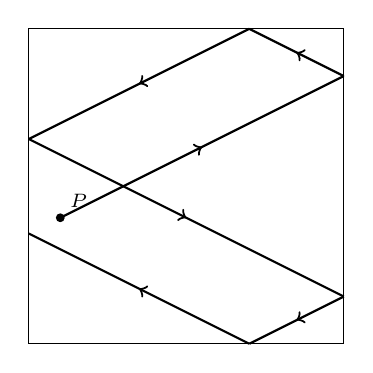
\begin{tikzpicture}[scale=0.8,
    every node/.style={font=\scriptsize},
    path/.style={decoration={markings,mark=at position 0.5 with {\arrow{>}}},postaction={decorate}, thick}]
    % Square boundaries
    \def\sqsize{5}
    \draw (0,0) rectangle (\sqsize,\sqsize);

    % Define path points
    \coordinate (P0) at (0.5, 2);
    \coordinate (P1) at (5, 4.25);
    \coordinate (P2) at (3.5, 5);
    \coordinate (P3) at (0, 3.25);
    \coordinate (P4) at (5, 0.75);
    \coordinate (P5) at (3.5, 0);
    \coordinate (P6) at (0, 1.75);
    % Add one more point for continuation if desired
    % P6=(0,1.75), vx=1, vy=0.5 (reflected L)
    % Hit R (x=5): dt=(5-0)/1=5. y=1.75+0.5*5 = 1.75+2.5 = 4.25. P7=(5,4.25) which is P1.
    \coordinate (P7) at (5, 4.25);


    % Draw path segments with arrows
    \draw[path] (P0) -- (P1);
    \draw[path] (P1) -- (P2);
    \draw[path] (P2) -- (P3);
    \draw[path] (P3) -- (P4);
    \draw[path] (P4) -- (P5);
    \draw[path] (P5) -- (P6);
    % \draw[path] (P6) -- (P7); % Example of continuation

    % Label starting point
    \fill (P0) circle (2pt) node[above right] {$P$};
\end{tikzpicture}
\caption{Path of a light ray reflecting inside a square, similar to Figure 4 in Stein \& Shakarchi. This illustrates how a path might evolve through multiple reflections. The properties of such paths are related to number theory and ergodic theory.}
\label{fig:billiards}
\end{figure}

\subsection*{Mathematical Formulation of Billiard Paths and Impact Sequences}
The dynamics in $S = [0,1]^2$ are analyzed by "unfolding" the path into a line $\mathbf{P}(t) = (X(t),Y(t)) = \mathbf{p}_0 + t\mathbf{v}$ in $\R^2$, where $\mathbf{p}_0=(x_0,y_0)$ is the initial position and $\mathbf{v}=(v_x,v_y)$ is the velocity. The position $(x(t),y(t)) \in S$ is $x(t)=f^*(X(t))$, $y(t)=f^*(Y(t))$, where the "folding map" $f^*: \R \to [0,1]$ is defined by $f^*(Z) = \langle Z \rangle$ if $\lfloor Z \rfloor$ is even, and $f^*(Z) = 1-\langle Z \rangle$ if $\lfloor Z \rfloor$ is odd.

Consider successive impacts on the vertical side $x=1$ (assuming $v_x>0$, particle starts near $x=0$). These occur when $X(t_k)=k$ for $k \in \N$ (appropriately indexed). Then $t_k = (k-x_0)/v_x$.
The corresponding $Y$-coordinates in the unfolded plane are $Y_k = y_0 + v_y t_k = y_0 + \frac{v_y}{v_x}(k-x_0)$.
Let $\alpha = v_y/v_x$ be the slope. Then $Y_k = \alpha k + (y_0 - \alpha x_0)$.
The sequence of $y$-impact coordinates in $S$ is $\{y_k^*\}_{k}$, where $y_k^* = f^*(Y_k)$.
The underlying sequence $Z_k = Y_k = \alpha k + \delta$ (with $\delta = y_0 - \alpha x_0$) is equidistributed modulo 1 if $\alpha \notin \Q$.
The mapping $f^*$ preserves equidistribution. For any continuous test function $g:[0,1]\to\R$, the limit of averages is:
$$ \lim_{K\to\infty} \frac{1}{K} \sum_{k=1}^K g(f^*(Z_k)) = \mathbb{E}[g(f^*(Z))]. $$
This expectation can be evaluated by considering the joint equidistribution of $(Z_k \pmod 1, \lfloor Z_k \rfloor \pmod 2)$ in $[0,1) \times \{0,1\}$ (if $\alpha \notin\Q$). This implies that terms with $\lfloor Z_k \rfloor$ even and odd each occur with asymptotic frequency $1/2$.
$$ \mathbb{E}[g(f^*(Z))] = \frac{1}{2}\mathbb{E}[g(\langle Z \rangle) | \lfloor Z \rfloor \text{ even}] + \frac{1}{2}\mathbb{E}[g(1-\langle Z \rangle) | \lfloor Z \rfloor \text{ odd}]. $$
Since $\langle Z \rangle$ is equidistributed in $[0,1)$ irrespective of the parity of $\lfloor Z \rfloor$ for irrational $\alpha$, this simplifies to:
$$ \mathbb{E}[g(f^*(Z))] = \frac{1}{2}\int_0^1 g(y)dy + \frac{1}{2}\int_0^1 g(1-y)dy. $$
As $\int_0^1 g(1-y)dy = \int_0^1 g(u)du$ (with $u=1-y$), the expression becomes $\int_0^1 g(y)dy$.
Thus, if $\alpha=v_y/v_x$ is irrational, the sequence of $y$-coordinates of impact on vertical sides is equidistributed on $[0,1]$. A symmetric argument applies for $x$-coordinates of impact on horizontal sides, using the slope $v_x/v_y$. The $\gamma$ in the main text refers to such an effective slope ratio.


\section{Conclusion}

Weyl's Equidistribution Theorem is a cornerstone result with implications in number theory, dynamical systems, and beyond. Its proof is a testament to the power of Fourier analysis, particularly:
\begin{itemize}
    \item The use of exponential functions $e^{2\pi i k x}$ as a basis.
    \item The principle of approximating general functions (continuous, Riemann integrable) by simpler ones (trigonometric polynomials, step functions) for which the result is easier to establish.
\end{itemize}
Weyl's Criterion further solidifies this connection, framing equidistribution entirely in terms of the limiting behavior of exponential sums, which are essentially discrete Fourier transforms. This interplay between continuous and discrete, and between number theory and analysis, is what makes the subject so rich and fascinating.


\begin{thebibliography}{9}

\bibitem{SteinShakarchi2003}
Stein, E. M., \& Shakarchi, R. (2003). \textit{Fourier Analysis: An Introduction} (Princeton Lectures in Analysis, Vol. I). Princeton University Press.

\bibitem{Korner1988}
Körner, T. W. (1988). \textit{Fourier Analysis}. Cambridge University Press.

\bibitem{WikipediaEquidistributed}
Wikipedia contributors. (n.d.). Equidistributed sequence. In \textit{Wikipedia, The Free Encyclopedia}. Retrieved May 26, 2025, from \url{https://en.wikipedia.org/wiki/Equidistributed_sequence}

\end{thebibliography}

\end{document}
